\documentclass{article}
\usepackage[utf8]{inputenc}
\usepackage[slovene]{babel}
\usepackage{graphicx}
\usepackage{subfigure}


\newcommand{\program}{Finanča matematika} 
\newcommand{\imeavtorja}{Anja Plesec} % ime avtorja
\newcommand{\imementorja}{prof.~dr.~ Sergio Cabello Justo, \\ asist. Gašper Domen Romih}
\newcommand{\naslovdela}{Gradientni spust}
\newcommand{\letnica}{2022}

\begin{document}

\thispagestyle{empty}
\noindent{\large
UNIVERZA V LJUBLJANI\\[1mm]
FAKULTETA ZA MATEMATIKO IN FIZIKO\\[5mm]
\program\ -- 2.~stopnja}
\vfill

\begin{center}{\large
\imeavtorja\\[2mm]
{\bf \naslovdela}\\[10mm]
Kratko poročilo pri predmetu Matematika z računalnikom\\[1cm]
Mentor: \imementorja}
\end{center}
\vfill

\noindent{\large
Ljubljana, \letnica}
\pagebreak

\newpage


\section{Gradientni spust}
Gradientni spust je iterativna metoda za iskanje lokalnega minimuma funkcije. 


Cilj je napisati algoritem s čim manj iteracij.



Splošen algoritem:
\begin{itemize}
\item{Izberemo začetno točko $x_0 \in R $ }
\item{Za $t  \geq 0$ predpostavimo, da poznamo $x_0,x_1, \ldots ,x_t $. Naslednji člen določimo s pomočjo enačbe: 
\[ x_{t+1}=x_t -  \eta \cdot \nabla f(x_t), \] 
kjer $ \eta$ predstavlja t.i. learning rate, $\nabla f(x_t) $ pa gradient funkcije $f$ v točki $x_t$}
\item{Končamo in vrnemo zadnjo iteracijo.}
\end{itemize}


Težava, ki se pojavi pri tem algoritmu je ustrezna dolžina koraka. Najraje bi delali velike korake v upanju na manjše število iteracij. Druga težava pa je ustrezna izbira začetne točke $x_0$, ki ni predaleč od optimalne rešitve.

\section{Dosedanje delo}
Gradientni spust doseže optimalno vrednost tako, da na začetku algoritma dela velike korake, ko pa se bliža optimalni vrednosti(minimumu) pa so koraki vedno manjši. To lastnost algoritma lahko potrdita tudi slika 1 in 2. Na prvi sliki torej vidimo, da pet dodatnih iteracij zelo vpliva na premico, saj gledamo razliko med 5 in 10 iteracij, med tem ko na drugi sliki, kjer gledamo razliko med 95 in 100 iteracij, skoraj ni razlike, saj so koraki, ki jih delamo vedno manjši. 

\begin{figure}[!htb]
   \begin{minipage}{0.6\textwidth}
     \centering
     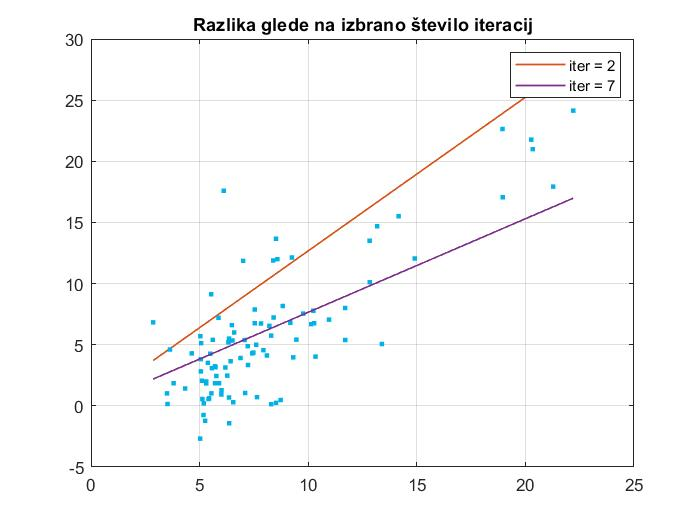
\includegraphics[width=1\linewidth]{premica_iter1}
     \caption{Število iteracij je 5 in 10}\label{Fig:Data1}
   \end{minipage}\hfill
   \begin{minipage}{0.6\textwidth}
     \centering
     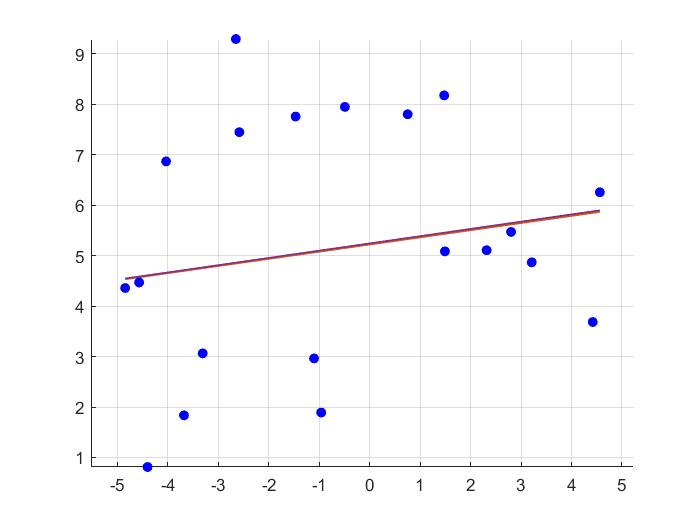
\includegraphics[width=1\linewidth]{premica_iter2}
     \caption{Število iteracij je 95 in 100}\label{Fig:Data2}
   \end{minipage}
\end{figure}

Izvedla sem poskus, kjer sem spreminjala začetne pogoje in opazovala koliko iteracij je potrebno da se približa optimalni rešitvi. V primeru a) sem vzela za parametra naklon in konstanta kar vrednost 1. Ko izvedemo 90 iteraij se zadnja iteracija dobro približa začetni rešitvi. Pri primeru b) sem vzela naklon = -20 in konst = 50


\begin{figure}
    \centering
    \subfigure[naklon = 1, konst = 1]{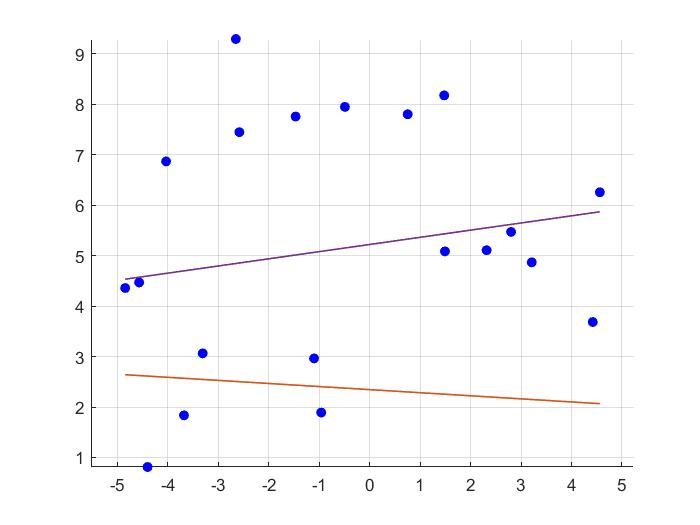
\includegraphics[width=0.45\textwidth]{premica_zp2.jpg}} 
    \subfigure[naklon = -20, konst = 50]{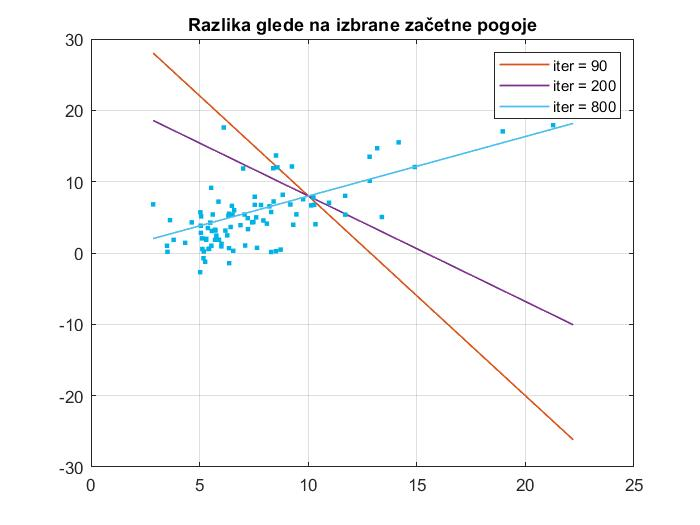
\includegraphics[width=0.45\textwidth]{premica_zp1.jpg}} 
    \subfigure[naklon = -200, konst = 500]{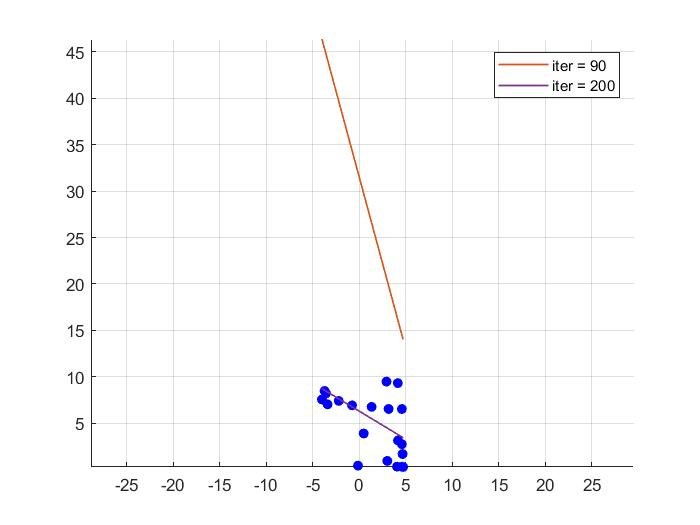
\includegraphics[width=0.45\textwidth]{premica_zp3.jpg}}
    \caption{Konvergenca pri različnih začetnih pogojih}
    \label{fig:foobar}
\end{figure}



\end{document}